
If the equation of the plane is given by
\begin{align}
\vec{n}^T\vec{x} = 1,
\end{align}
\begin{align}
\myvec{1&1&-1 \\ 6&4&-5 \\ -4&-2&3} \vec{n} &= \myvec{1\\1\\1}
\end{align}
Row reducing the augmented matrix, 
\begin{align}
\myvec{1 & 0 & -0.5 & -1.5\\0 & 1 & -0.5 & 2.5\\0 & 0 & 0 & 0}
\end{align}
which yields the  equation of the line
\begin{align}
\vec{x} &= \myvec{1 \\ 6 \\ -4}+\lambda\myvec{0 \\ -2 \\2}
\end{align}
and is plotted in Fig. \ref{linform/38/a/Plot of the line}.
\begin{figure}[ht]
\centering
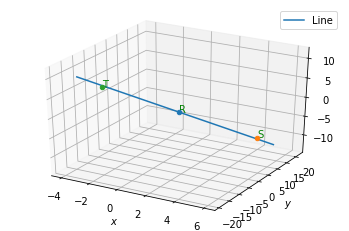
\includegraphics[width=\columnwidth]{solutions/su2021/2/36/a/download (5).png}
\caption{plot of the line}
\label{linform/38/a/Plot of the line}
\end{figure}


